\documentclass[journal]{IEEEtran}
\ifCLASSINFOpdf
\usepackage[pdftex]{graphicx}
\else
\fi
\usepackage{amsmath}
\usepackage{amssymb}
\usepackage{amsthm}
\usepackage{bm}
\usepackage{mathrsfs}
\hyphenation{La-grange La-grang-ian dy-nam-ics}
\newcommand{\bma}[1]{\left[\begin{array}{#1}}
\newcommand{\ema}{\end{array}\right]}
\newcommand{\trans}{{\ensuremath{\mathsf{T}}}} % transpose
\newcommand{\utimes}{ {\raisebox{-0.6ex}{ \kern-1.0ex\raisebox{0.6ex}{ \small $\mathsf{v}$}}} } % 
\newcommand{\onehalf}{\mbox{$\textstyle{\frac{1}{2}}$}}
\DeclareMathAlphabet{\mbf}{OT1}{ptm}{b}{n}
\newcommand{\mbs}[1]{{\boldsymbol{#1}}}
\newcommand{\mbfbar}[1]{{\bar{\mbf{#1}}}}
\newcommand{\mbfhat}[1]{{\hat{\mbf{#1}}}}
\newcommand{\mbftilde}[1]{{\tilde{\mbf{#1}}}}
\newcommand{\mbsbar}[1]{{\bar{\boldsymbol{#1}}}}
\newcommand{\mbshat}[1]{{\hat{\boldsymbol{#1}}}}
\newcommand{\mbstilde}[1]{{\tilde{\boldsymbol{#1}}}}
\newcommand{\pspace}{\mathbb{P}} 
\newcommand{\ura}[1]{{\underrightarrow{{#1}}}}
\newcommand{\vectrix}[1]{\ensuremath \underrightarrow{\boldsymbol{\mathcal{F}}}_{#1}}
\def\fdota{{\raisebox{-2pt}{\LARGE $\cdot$}}}
\def\fdotb{{\raisebox{-0.6ex}{ \kern0.2ex\raisebox{0.8ex}{\tiny $\hspace*{-1ex}\circ$}}}}
\def\fddota{{\raisebox{-2pt}{\LARGE $\cdot\hspace*{-0.2ex}\cdot$}}}
\def\fddotb{{\raisebox{-0.6ex}{ \kern0.2ex\raisebox{0.8ex}{\tiny $\hspace*{-1ex}\circ\circ$}}}}
\newcommand{\fdot}[1]{{^{\fdota{\mbox{\footnotesize${#1}$}}}}}
\newcommand{\fddot}[1]{{^{\fddota{\mbox{\footnotesize${#1}$}}}}}
\newcommand{\beq}{\begin{equation}}
\newcommand{\eeq}{\end{equation}}
\newcommand{\bdis}{\begin{displaymath}}
\newcommand{\edis}{\end{displaymath}}
\newcommand{\beqarray}{\begin{eqnarray}}
\newcommand{\eeqarray}{\end{eqnarray}}
\newcommand{\beqarraynn}{\begin{eqnarray*}}
\newcommand{\eeqarraynn}{\end{eqnarray*}}

\begin{document}

\title{Quad-Rotor Helicopter Final Project}

\author{{Gregory Miller 50760004}}

\markboth{AER 540 -- Intermediate Dynamics, Fall 2014}
{}

\maketitle

\begin{abstract}
This document provides a brief introduction to quad-rotor helicopters and then derives the kinematics and dynamics model of a quad-rotor helicopter, or in other words, its equations of motion. Using the model, simulations are performed in Matlab to analyze the helicopter's trajectory over time under different conditions. 
\end{abstract}

\IEEEpeerreviewmaketitle

\section{Introduction and Motivation}
\label{sec:intro_section}

\IEEEPARstart{A}{}quad-rotor helicopter is a flying device that has four horizontal spinning rotors which produce the upward thrust needed to lift the center piece, or body of the helicopter, into the air. See Figure \ref{fig:quad_intro} below, courtesy of Reference \cite{quad_intro}, for a visual example of a quad-rotor helicopter:

\begin{figure}[ht]
    \centering
        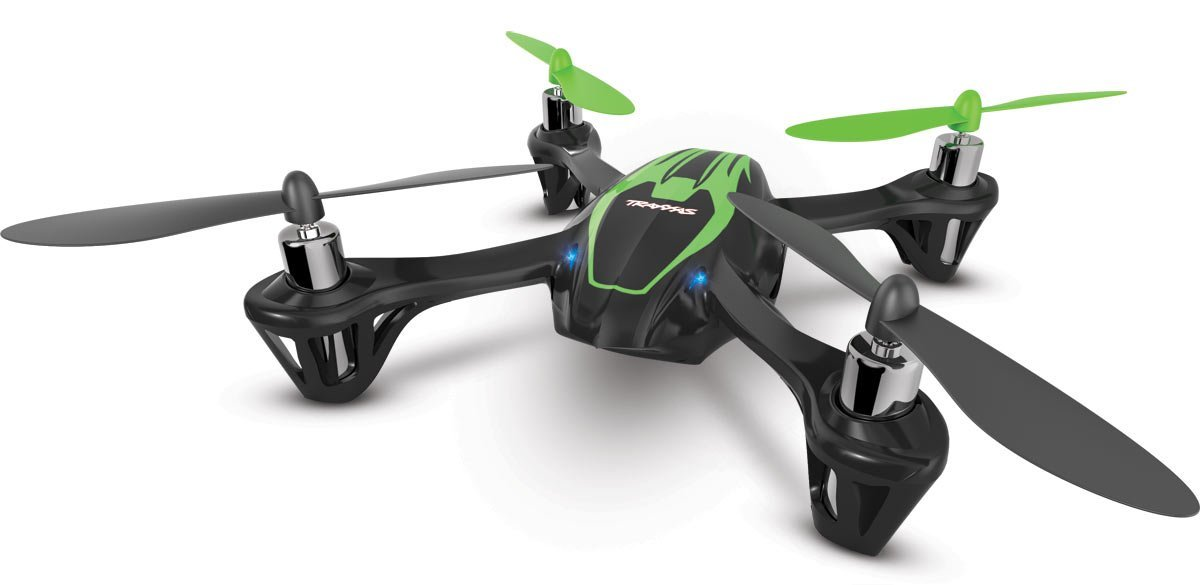
\includegraphics[width=.30\textwidth]{quad_intro}
    \caption{A visual example of a quad-rotor helicopter. Notice the four rotors.}
    \label{fig:quad_intro}
\end{figure}

 The purpose of this course project is to model the kinematics and dynamics of a quad-rotor helicopter. The inspiration for this project came from the Michigan Autonomous Aerial Vehicles Club (MAAV). Every year, the club designs and constructs a quad-rotor helicopter to compete in a competition the subsequent August. In this competition, the goal is to have the quad-rotor helicopter autonomously navigate its own way through an obstacle course. As no human navigation input into the helicopter is allowed, its processor must use controllers that can successfully command the helicopter's actuators, i.e., the four spinning rotors, to direct the helicopter through its path. As such, it would be useful to model the quad-rotor helicopter's kinematics and dynamics as this information is needed in order to design the controllers to produce steady and stable flight through any desired trajectory.   

\section{Kinematics of the Quad-Rotor Helicopter}
\label{sec:kinematics_section}

Kinematics refers to the geometry of motion of a moving object. The motion of the quad-rotor helicopter is going to be determined by the locations and directions of the external forces that are applied to its body. Arguably the most important of these forces are the four lift forces produced by the helicopter's four rotors. These forces lift the helicopter into the air and propel it forward. In fact, the only means in which the helicopter has control over its motion is through its knowledge of the locations of these forces and its orientation in space. As such, knowing the kinematics of the four rotors is necessary. Figure \ref{fig:top_view} at the top of the next column shows the relevant kinematics information for the helicopter from a top-down perspective.

\begin{figure}[ht]
    \centering
        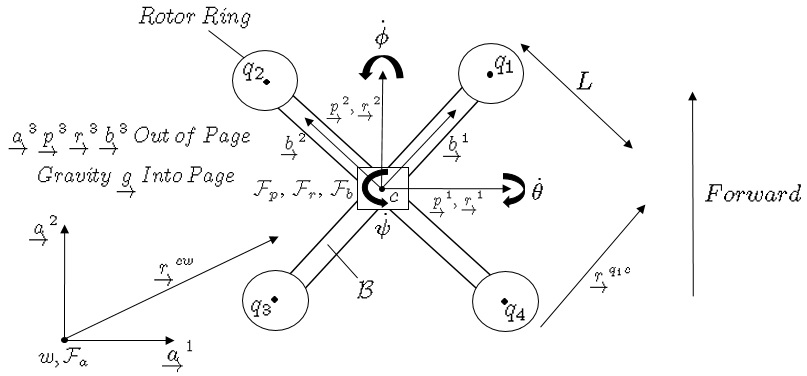
\includegraphics[width=.50\textwidth]{top_view}
    \caption{The relevant kinematics information of the quad-rotor helicopter}
    \label{fig:top_view}
\end{figure}

Note that the helicopter is taken as the body $\mathcal{B}$, $w$ is an unforced particle that coincides with the origin of the inertial frame $\mathcal{F}_a$, and point $c$ is the center of mass of the helicopter, taken to be its geometric center as the helicopter is symmetric and assumed to have uniform densities. Note the locations of the four rotors in Figure \ref{fig:top_view}, marked by the $q_i$ points where $i=1,\ldots,4$. The goal is to compute the velocities of the four rotors, i.e., $\underrightarrow{v}^{q_iw/a} $. Computing their accelerations, $\underrightarrow{a}^{q_iw/a}$, is unnecessary as a Newton-Euler approach will be used to determine the equations of motion for the helicopter. Next, Figure \ref{fig:rotor_arm} displays a close-up view of a rotor and its associated arm:

\begin{figure}[ht]
    \centering
        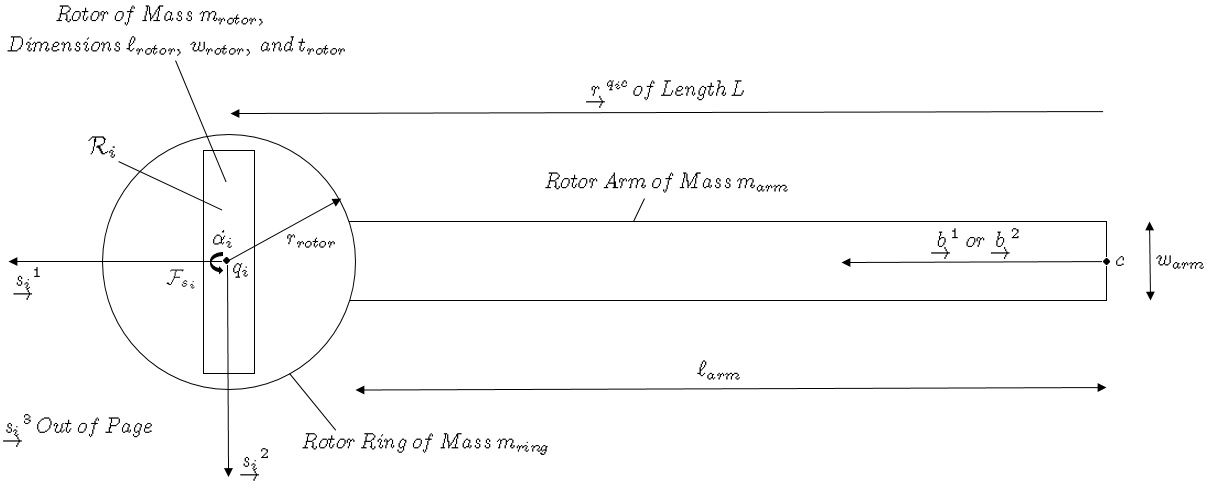
\includegraphics[width=.50\textwidth]{rotor_arm}
    \caption{Close-up view of a rotor and its associated arm}
    \label{fig:rotor_arm}
\end{figure}

Note that the rotors are taken as bodies $\mathcal{R}_i$, where $i=1,\dots,4$. Thus, the entire system is denoted as $\mathcal{S}=\mathcal{B}+\mathcal{R}_1+\mathcal{R}_2+\mathcal{R}_3+\mathcal{R}_4$. With Figures \ref{fig:top_view} and \ref{fig:rotor_arm} in mind, the kinematics analysis can begin. Note that there are four frames shown in Figure \ref{fig:top_view}. They are summarized in the following list:

\begin{enumerate}
\item As mentioned previously, the frame $\mathcal{F}_a$ is the inertial frame. It is the frame that quantities will be computed with respect to. 
\item The pitch (p) frame $\mathcal{F}_p$. This frame is created by rotating $\mathcal{F}_a$ about $\underrightarrow{a}^1$ by the pitch angle $\theta$. This frame is coincident with the quad-rotor helicopter body and the basis vector $\underrightarrow{p}^2$ remains fixed in the plane created by the four rotors.
\item The roll (r) frame $\mathcal{F}_r$. This frame is created by rotating $\mathcal{F}_p$ about $\underrightarrow{p}^2$ by the roll angle $\phi$. This frame is coincident with the quad-rotor helicopter body and the basis vector $\underrightarrow{r}^1$ remains fixed in the plane created by the four rotors.
\item The yaw, or body $\mathcal{B}$ (b), frame $\mathcal{F}_b$. This frame is created by rotating $\mathcal{F}_r$ about $\underrightarrow{r}^3$ by the yaw angle $\psi$. This frame is fixed to the quad-rotor helicopter body and the basis vectors $\underrightarrow{b}^1$ and $\underrightarrow{b}^2$ remain fixed to the helicopter's arms. 
\end{enumerate}

For the Direction-Cosine Matrix (DCM) representation, Euler-angle rotation matrices will be used because they are well-suited for the pitch-roll-yaw frame designations described above and because the quad-rotor helicopter is never expected to produce the kinematic singularity associated with Euler-angle rotation matrices, or in other words, rotate $90$ degrees about any one axis. 

That being said, the four frames undergo a 1-2-3 Euler-angle sequence. Equation \ref{eq:eulerseq} below provides the formal representation of this sequence:

\begin{equation}
	\mathcal{F}_a \xrightarrow[\underline{C_1}(\theta)]{} \mathcal{F}_p \xrightarrow[\underline{C_2}(\phi)]{} \mathcal{F}_r \xrightarrow[\underline{C_3}(\psi)]{} \mathcal{F}_b
	\label{eq:eulerseq}
\end{equation}

The overall DCM matrix is computed next in Equations \ref{eq:dcmbase} and \ref{eq:dcm}:

\begin{equation}
	\underline{C}_{ba}=\underline{C}_{br}\underline{C}_{rp}\underline{C}_{pa}=\underline{C_3}{(\psi)}\underline{C_2}{(\phi)}\underline{C_1}{(\theta)}
	\label{eq:dcmbase}
\end{equation}
\begin{equation}
	\underline{C}_{ba}=\left[ \begin{array}{ccc}
	c_{\phi}c_{\psi} & c_{\theta}s_{\psi}+s_{\theta}s_{\phi}c_{\psi} & s_{\theta}s_{\psi}-c_{\theta}s_{\phi}c_{\psi} \\
	-c_{\phi}s_{\psi} & c_{\theta}c_{\psi}-s_{\theta}s_{\phi}s_{\psi} & s_{\theta}c_{\psi}+c_{\theta}s_{\phi}s_{\psi} \\
	s_{\phi} & -s_{\theta}c_{\phi} & c_{\theta}c_{\phi} \\
	\end{array} \right]
	\label{eq:dcm}
\end{equation}

Looking at Figure \ref{fig:rotor_arm}, one can see that there are additional frames $\mathcal{F}_{s_i}$ that are associated with each of the four rotors where $i=1,\ldots,4$. These frames are created by rotating $\mathcal{F}_b$ about $\underrightarrow{b}^3$ by the rotor-rotation angles $\alpha_i$. Hence the rotations are described by the $\underline{C}_{s_ib}=\underline{C_3}(\alpha_i)$ DCM's. In other words, each rotor is able to rotate independently of the other rotors. The frames $\mathcal{F}_{s_i}$ are fixed to each of the rotor bodies and each basis vector $\underrightarrow{s_i}^1$ remains aligned with its affiliated rotor-length axis. The DCM's $\underline{C}_{s_ia}$ do not need to be explicitly computed because they will not be used in the model of the helicopter.

Next, the angular velocity of $\mathcal{F}_b$ with respect to $\mathcal{F}_a$, $\underrightarrow{\omega}^{ba}$, is computed. Note that angular velocities of the frames with respect to each other add, as stated in Equation \ref{eq:angadd}:

\begin{equation}
	\underrightarrow{\omega}^{ba}=\underrightarrow{\omega}^{br}+\underrightarrow{\omega}^{rp}+\underrightarrow{\omega}^{pa}
	\label{eq:angadd}
\end{equation}

Using Poisson's Equation, Equation \ref{eq:poisson}, the following can be stated concerning the components of three angular velocities on the right-hand side of Equation \ref{eq:angadd}, stated in Equations \ref{eq:angcomp1} through \ref{eq:angcomp3}:

\begin{equation}
	\underline{\dot{C}}_{yx}=-\underline{\omega}^{yx\times}_y\underline{C}_{yx}
	\label{eq:poisson}
\end{equation}
\begin{equation}
	\underline{\dot{C}}_1(\theta)=-\dot{\theta}\underline{\mathbf{1}}^{\times}_1\underline{C}_1(\theta) \xrightarrow[]{} \underline{\omega}^{pa}_p=\dot{\theta}\underline{\mathbf{1}}_1
	\label{eq:angcomp1}
\end{equation}
\begin{equation}
	\underline{\dot{C}}_2(\phi)=-\dot{\phi}\underline{\mathbf{1}}^{\times}_2\underline{C}_2(\phi) \xrightarrow[]{} \underline{\omega}^{rp}_r=\dot{\phi}\underline{\mathbf{1}}_2
	\label{eq:angcomp2}
\end{equation}
\begin{equation}
	\underline{\dot{C}}_3(\psi)=-\dot{\psi}\underline{\mathbf{1}}^{\times}_3\underline{C}_3(\psi) \xrightarrow[]{} \underline{\omega}^{br}_b=\dot{\psi}\underline{\mathbf{1}}_3
	\label{eq:angcomp3}
\end{equation}

Adding the angular velocity components together and resolving the results in frame $\mathcal{F}_b$ in Equations \ref{eq:angaddresb1} through \ref{eq:angaddresb4} provides an explicit expression for $\underrightarrow{\omega}^{ba}$:

\begin{equation}
	\underrightarrow{\omega}^{ba}=\underrightarrow{\mathcal{F}}^T_b\underline{\omega}^{br}_b+\underrightarrow{\mathcal{F}}^T_r\underline{\omega}^{rp}_r+\underrightarrow{\mathcal{F}}^T_p\underline{\omega}^{pa}_p
	\label{eq:angaddresb1}
\end{equation}
\begin{equation}
\underrightarrow{\omega}^{ba}=\underrightarrow{\mathcal{F}}^T_b[\underline{C_3}(\psi)\underline{C_2}(\phi)\underline{\mathbf{1}}_1+\underline{C_3}(\psi)\underline{\mathbf{1}}_2+\underline{\mathbf{1}}_3]	\left[ \begin{array}{c}
	\dot{\theta}  \\
	\dot{\phi}  \\
	\dot{\psi} \\
	\end{array} \right]
\label{eq:angaddresb2}
\end{equation}
\begin{equation}
\underrightarrow{\omega}^{ba}=\underrightarrow{\mathcal{F}}^T_b
\underline{S}^{ba}_b\underline{\dot{\theta}}^{ba}	
\label{eq:angaddresb3}
\end{equation}
\begin{equation}
\underrightarrow{\omega}^{ba}=\underrightarrow{\mathcal{F}}^T_b
	\left[ \begin{array}{c}
	c_{\phi}c_{\psi}\dot{\theta}+s_{\psi}\dot{\phi}  \\
	-c_{\phi}s_{\psi}\dot{\theta}+c_{\psi}\dot{\phi}  \\
	s_{\phi}\dot{\theta}+\dot{\psi} \\
	\end{array} \right]
\label{eq:angaddresb4}
\end{equation}

Note that the component matrix of Euler-angle rates is denoted as $\dot{\theta}^{ba}$ in Equation \ref{eq:angaddresb3}. Next, the angular velocities $\underrightarrow{\omega}^{s_ia}$ are easily computed by expanding upon the angular velocity $\underrightarrow{\omega}^{ba}$ as done in Equations \ref{eq:angvelsia1} and \ref{eq:angvelsia2}:

\begin{equation}
\underrightarrow{\omega}^{s_ia}=\underrightarrow{\omega}^{s_ib}+\underrightarrow{\omega}^{ba}=\underrightarrow{\mathcal{F}}^T_b[\underline{C^T_3}(\alpha_i)\left[ \begin{array}{c}
	0  \\
	0 \\
	\dot{\alpha_i} \\
	\end{array} \right]+\underline{\omega}^{ba}_b]
\label{eq:angvelsia1}
\end{equation} 

\begin{equation}
\underrightarrow{\omega}^{s_ia}=\underrightarrow{\mathcal{F}}^T_b[\left[ \begin{array}{c}
		0  \\
		0 \\
		\dot{\alpha_i} \\
		\end{array} \right]+\underline{\omega}^{ba}_b]
\label{eq:angvelsia2}
\end{equation} 

Moving on, as is clear in Figure \ref{fig:top_view}, the following position vector relation for rotor $\mathcal{R}_1$, Equation \ref{eq:posvect}, holds:

\begin{equation}
	\underrightarrow{r}^{q_1w}=	\underrightarrow{r}^{cw}+	\underrightarrow{r}^{q_1c}
	\label{eq:posvect}
\end{equation}

Noting that the scalar positions $x_c$, $y_c$, and $z_c$, which are not constant, locate the center of mass $c$ relative to unforced particle $w$ resolved in frame $\mathcal{F}_a$, and that $L$, which is constant, locates point $q_1$ relative to $c$ parallel to the $\underrightarrow{b}^1$ axis, Equation \ref{eq:posvectcomp} provides the components of the two position vectors shown in the right-hand side of Equation \ref{eq:posvect}:

\begin{equation}
	\underrightarrow{r}^{q_1w}=\underrightarrow{\mathcal{F}}^T_a
		\left[ \begin{array}{c}
		x_c \\
		y_c \\
		z_c \\
		\end{array} \right]+\underrightarrow{\mathcal{F}}^T_b
				\left[ \begin{array}{c}
				L \\
				0 \\
				0 \\
				\end{array} \right]			
	\label{eq:posvectcomp}
\end{equation}

Next, the velocity $\underrightarrow{v}^{q_1w/a}$ is computed in Equations \ref{eq:vel1} through \ref{eq:vel5}. Note the use of the Transport Theorem, the angular velocity $\underrightarrow{\omega}^{ba}$ stated in Equation \ref{eq:angaddresb3}, and the fact that $L$ is constant:

\begin{equation}
	\underrightarrow{v}^{q_1w/a}=\underrightarrow{r}^{q_1w\cdot{a}}=\underrightarrow{r}^{cw\cdot{a}}+\underrightarrow{r}^{q_1c\cdot{a}}
	\label{eq:vel1}
\end{equation}
\begin{equation}
	\underrightarrow{v}^{q_1w/a}=\underrightarrow{\mathcal{F}}^T_a\underline{\dot{r}}^{cw}_a+\underrightarrow{r}^{q_1c\cdot{b}}+	\underrightarrow{\omega}^{ba}\times\underrightarrow{r}^{q_1c}
	\label{eq:vel2}
\end{equation}
\begin{equation}
	\underrightarrow{v}^{q_1w/a}=\underrightarrow{\mathcal{F}}^T_a\left[ \begin{array}{c}
			\dot{x_c} \\
			\dot{y_c} \\
			\dot{z_c} \\
			\end{array} \right]+\underrightarrow{\mathcal{F}}^T_b\underline{0}+\underrightarrow{\mathcal{F}}^T_b\underline{\omega}^{ba\times}_b\underline{r}^{q_1c}_b
	\label{eq:vel3}
\end{equation}
\begin{equation}
	\underrightarrow{v}^{q_1w/a}=\underrightarrow{\mathcal{F}}^T_b\underline{C}_{ba}\left[ \begin{array}{c}
			\dot{x_c} \\
			\dot{y_c} \\
			\dot{z_c} \\
			\end{array} \right]+\underrightarrow{\Delta}		
	\label{eq:vel4}
\end{equation}
\begin{equation}
	\underrightarrow{\Delta}=\underrightarrow{\mathcal{F}}^T_b\left[    \begin{array}{c}
						0 \\
			(s_{\phi}\dot{\theta}+\dot{\psi})L \\
			(c_{\phi}s_{\psi}\dot{\theta}-c_{\psi}\dot{\phi})L \\
						\end{array} \right]		
	\label{eq:vel5}
\end{equation}
Note that $\underline{C}_{ba}$ was provided in Equation \ref{eq:dcm}. Last, the acceleration $\underrightarrow{a}^{q_1w/a}$ is computed in Equations \ref{eq:acc1} and \ref{eq:acc2}. Note the use of the Transport Theorem and the angular velocity $\underrightarrow{\omega}^{ba}$ stated in Equation \ref{eq:angaddresb3}:

\begin{equation}
	\underrightarrow{a}^{q_1w/a}=\underrightarrow{v}^{q_1w/a\cdot{a}}=\underrightarrow{\mathcal{F}}^T_a\underline{\ddot{r}}^{cw}_a+\underrightarrow{\Delta}^{\cdot{a}}
	\label{eq:acc1}
\end{equation}
\begin{equation}
	\underrightarrow{a}^{q_1w/a}=\underrightarrow{\mathcal{F}}^T_b\underline{C}_{ba}\left[ \begin{array}{c}
				\ddot{x_c} \\
				\ddot{y_c} \\
				\ddot{z_c} \\
				\end{array} \right]+\underrightarrow{\mathcal{F}}^T_b[\underline{\dot{\Delta}}_b+\underline{\omega}^{ba\times}_b\underline{\Delta}_b]
	\label{eq:acc2}
\end{equation}

Computing the acceleration, the calculations of which are too cumbersome to write into this document, produces $\ddot{\theta}$, $\ddot{\phi}$, and $\ddot{\psi}$ terms. Note that $L$ is constant. These computations are easily extended to the other three rotors, $\mathcal{R}_2$, $\mathcal{R}_3$, and $\mathcal{R}_4$. Note, as mentioned previously, their accelerations will not be necessary as the model of the quad-rotor helicopter will be derived using a Newton-Euler approach, described in the next section. 

\section{Dynamics of the Quad-Rotor Helicopter}
Dynamics refers to the motion of an object under the influence of forces and moments. The dynamics of the quad-rotor helicopter will be derived using a clear, systematic approach. To begin, the first moment of mass of the helicopter relative to its center of mass $c$ is given by Equation \ref{eq:firstmoment}:

\begin{equation}
	\underrightarrow{c}^{\mathcal{S}c}=\int_{\mathcal{S}}^{} \underrightarrow{r}^{dm_{\mathcal{S}}c} dm_{\mathcal{S}}=m_{\mathcal{S}}\underrightarrow{r}^{cc}=\underrightarrow{0}
	\label{eq:firstmoment}
\end{equation} 

The mass of the entire helicopter system $\mathcal{S}$ (helicopter body $\mathcal{B}$ and four rotors $\mathcal{R}_i$) is $m_{\mathcal{S}}$ and $dm_{\mathcal{S}}$ is a differential mass element within the helicopter system $\mathcal{S}$. The first moment of mass relative to $c$ is equal to the zero vector because the position of the center of mass $c$ relative to itself is of course $\underrightarrow{0}$.  

Next, the second moment of mass of the helicopter relative to its center of mass $c$, excluding the second moments of mass of the four rotors, is given by Equations \ref{eq:Bsecmoment1} through \ref{eq:Bsecmoment5}:

\begin{equation}
	\underrightarrow{J}^{\mathcal{B}c}=\int_{\mathcal{B}}^{}
	(\underrightarrow{r}^{dm_{\mathcal{B}}c}\cdot\underrightarrow{r}^{dm_{\mathcal{B}}c}\underrightarrow{1}- \underrightarrow{r}^{dm_{\mathcal{B}}c}\underrightarrow{r}^{dm_{\mathcal{B}}c})dm_{\mathcal{B}}
	\label{eq:Bsecmoment1}
\end{equation} 

\begin{equation}
	\underrightarrow{J}^{\mathcal{B}c}=\underrightarrow{\mathcal{F}}^T_b\left[ \begin{array}{ccc}
					J^{\mathcal{B}c11}_b & 0 & 0\\
					0 & J^{\mathcal{B}c22}_b & 0\\
					0 & 0 & J^{\mathcal{B}c33}_b\\
					\end{array} \right]\underrightarrow{\mathcal{F}}_b
	\label{eq:Bsecmoment2}
\end{equation} 

\begin{equation}
	J^{\mathcal{B}c11}_b=\frac{1}{3}m_aw^2_a+\frac{1}{6}m_a(4\ell^2_a+w^2_a)+2m_rr^2_r+2m_rL^2
	\label{eq:Bsecmoment3}
\end{equation} 

\begin{equation}
	J^{\mathcal{B}c22}_b=J^{\mathcal{B}c11}_b
	\label{eq:Bsecmoment4}
\end{equation} 

\begin{equation}
	J^{\mathcal{B}c33}_b=\frac{1}{3}m_a(4\ell^2_a+w^2_a)+4m_rr^2_r+4m_rL^2
	\label{eq:Bsecmoment5}
\end{equation} 

The parameters $m_a$, $w_a$, and $\ell_a$ are the mass, width/thickness, and length respectively of the one of the four rotor arms. The parameters $m_r$ and $r_r$ are the mass and radius respectively of one of the four rotor rings (a thin-ring assumption is used). Last, the distance $L$ is of course the length from the center of mass $c$ to any of the four $q_i$ rotor points.   

The same statements can be made for each of the four rotors. The second moment of mass of each rotor relative to its (assumed) center of mass $q_i$ is given by Equations \ref{eq:Rsecmoment1} through \ref{eq:Rsecmoment5}:

\begin{equation}
	\underrightarrow{J}^{\mathcal{R}_iq_i}=\int_{\mathcal{R}_i}^{}
	(\underrightarrow{r}^{dm_{\mathcal{R}_i}q_i}\cdot\underrightarrow{r}^{dm_{\mathcal{R}_i}q_i}\underrightarrow{1}- \underrightarrow{r}^{dm_{\mathcal{R}_i}q_i}\underrightarrow{r}^{dm_{\mathcal{R}_i}q_i})dm_{\mathcal{R}_i}
	\label{eq:Rsecmoment1}
\end{equation} 

\begin{equation}
	\underrightarrow{J}^{\mathcal{R}_iq_i}=\underrightarrow{\mathcal{F}}^T_{s_i}\left[ \begin{array}{ccc}
					J^{\mathcal{R}_iq_i11}_{s_i} & 0 & 0\\
					0 & J^{\mathcal{R}_iq_i22}_{s_i} & 0\\
					0 & 0 & J^{\mathcal{R}_iq_i33}_{s_i}\\
					\end{array} \right]\underrightarrow{\mathcal{F}}_{s_i}
	\label{eq:Rsecmoment2}
\end{equation} 

\begin{equation}
	J^{\mathcal{R}_iq_i11}_{s_i}=\frac{1}{2}m_{\mathcal{R}_i}(\ell_r^2+t_r^2)
	\label{eq:Rsecmoment3}
\end{equation} 

\begin{equation}
	J^{\mathcal{R}_iq_i22}_{s_i}=\frac{1}{2}m_{\mathcal{R}_i}(w_r^2+t_r^2)
	\label{eq:Rsecmoment4}
\end{equation} 

\begin{equation}
	J^{\mathcal{R}_iq_i33}_{s_i}=\frac{1}{2}m_{\mathcal{R}_i}(\ell_r^2+w_r^2)
	\label{eq:Rsecmoment5}
\end{equation} 

The parameters $m_r$, $\ell_r$, $w_r$, and $t_r$ are the mass, length, width, and thickness respectively of the four rotors.

Reference \cite{dual_spin} provides the relationship between $\underline{J}^{\mathcal{R}_iq_i}_s$ and $\underline{J}^{\mathcal{R}_ic}_b$, that is, the second moment of mass of each rotor with respect to the helicopter center of mass $c$ resolved in the body $\mathcal{B}$ (b) frame. This relationship is stated in Equation \ref{eq:JRqsJRcb}:

\begin{equation}
\underline{J}^{\mathcal{R}_ic}_b=\underline{C^T_3}(\alpha_i)\underline{J}^{\mathcal{R}_iq_i}_{s_i}\underline{C_3}(\alpha_i)-m_{\mathcal{R}_i}\underline{r}^{q_ic\times}_b\underline{r}^{q_ic\times}_b 
\label{eq:JRqsJRcb}
\end{equation}

It should be noted that the $\underline{J}^{\mathcal{B}c}_b$ matrix in Equation \ref{eq:Bsecmoment2} is diagonal because it is resolved in the body $\mathcal{B}$ (b) frame and because the quad-rotor helicopter is symmetrical and assumed to have uniform densities. The matrix $\underline{J}^{\mathcal{R}_iq_i}_{s_i}$ in Equation \ref{eq:Rsecmoment2} is diagonal for the same reasons.  The components of both matrices were derived using second moment of mass tables found on the inside covers of Reference \cite{dynamics_book} and the "Parallel-Axis Theorem", also found in Reference \cite{dynamics_book} but on page $401$. This theorem is stated as Equation \ref{eq:paraxisth}:

\begin{equation}
J=J_G+md^2
\label{eq:paraxisth}
\end{equation} 

All values shown are scalar values. The parameter $J_G$ is the mass moment of inertia of an object about a specific axis that passes through its center of mass $G$, $J$ is the mass moment of inertia of the object about a different but parallel axis, $m$ is the mass of the object, and $d$ is the perpendicular distance between the two parallel axes.

A Newton-Euler approach is used to derive the equations of motion of the quad-rotor helicopter. This approach is chosen over the Lagrangian approach simply because the Newton-Euler approach appears to be less complicated. 

To begin, there are six forces acting upon the quad-rotor helicopter. First, there are four lift forces produced by the four rotors, which are each applied at the $q_i$ points and act in the positive $\underrightarrow{b}^3$ direction. Next, there is the weight of the entire system $\mathcal{S}$ (the helicopter body $\mathcal{B}$ plus the four rotors $\mathcal{R}_i$) which is applied at the center of mass $c$ and acts in the negative $\underrightarrow{a}^3$ direction. Last, a drag force is modeled which is assumed to be applied at the center of mass $c$ and it always acts in the negative direction of the velocity $\underrightarrow{v}^{cw/a}$. It is proportional to the speed of the helicopter, $|\underrightarrow{v}^{cw/a}|$. These forces are stated in Equations \ref{eq:force1} through \ref{eq:force3}:

\begin{equation}
\underrightarrow{f}^{\mathcal{S}}=(\sum_{i=1}^4\underrightarrow{f}^i)+\underrightarrow{f}^{\mathcal{S}g}+\underrightarrow{f}^{\mathcal{S}d}
\label{eq:force1}
\end{equation}
\begin{equation}
\underrightarrow{f}^{\mathcal{S}}=\underrightarrow{\mathcal{F}}^T_a[\underline{C}^T_{ba}\left[ \begin{array}{c}
				0 \\
				0 \\
				f^1+f^2+f^3+f^4 \\
				\end{array} \right]+\left[ \begin{array}{c}
								0 \\
								0 \\
								-m_{\mathcal{S}}g \\
								\end{array} \right]]+\underrightarrow{f}^{\mathcal{S}d}
\label{eq:force2}
\end{equation}
\begin{equation}
\underrightarrow{f}^{\mathcal{S}d}=-\frac{1}{2}C_{drag}\rho_{air}(\frac{A_{top}}{3})\sqrt{\dot{x}^2_c+\dot{y}^2_c+\dot{z}^2_c}\underrightarrow{\mathcal{F}}^T_a\left[ \begin{array}{c}
				\dot{x}_c \\
				\dot{y}_c \\
				\dot{z}_c \\
				\end{array} \right]
\label{eq:force3}
\end{equation}
Note that the mass of the entire system $\mathcal{S}$ is $m_{\mathcal{S}}$, $g$ is the acceleration due to gravity, $C_{drag}$ is the drag coefficient, $\rho_{air}$ is the density of the air, and $A_{top}$ is the top surface area of the helicopter. It needs to be noted that the surface-area term in drag force computations needs to be taken as the front-face surface area. However, it is complicated to compute this front-face surface area for the helicopter because its angular orientation is consistently changing. Hence, a simplification is made in that the front-face surface area is taken to be a constant fraction of the top surface area. Last, note that all of the differential mass elements' $dm_{\mathcal{S}}$ weights are integrated together to produce the weight force $\underrightarrow{f}^{\mathcal{S}g}$.

Next, since the only forces that do not act on the center of mass $c$ are the four lift forces $\underrightarrow{f}^i$, these are the only four forces that produce moments on the helicopter system $\mathcal{S}$ relative to its center of mass $c$. These moments are stated in Equation \ref{eq:moments}:

\begin{equation}
\underrightarrow{m}^{\mathcal{S}c}=(\sum_{i=1}^4\underrightarrow{r}^{q_ic}\times\underrightarrow{f}^i)=\underrightarrow{\mathcal{F}}^T_b\left[ \begin{array}{c}
				Lf^2-Lf^4 \\
				-Lf^1+Lf^3 \\
				0 \\
				\end{array} \right]
\label{eq:moments}
\end{equation}
All of the moments due to the differential mass elements' $dm_{\mathcal{S}}$ weights are canceled out when integrated together because the helicopter system is symmetrical and assumed to have uniform densities. 

The linear momentum of the helicopter system $\mathcal{S}$ relative to the unforced particle $w$ with respect to frame $\mathcal{F}_a$ is displayed in Equation \ref{eq:linmomentum} at the top of the next column.

\begin{equation}
\underrightarrow{p}^{\mathcal{S}w/a}=m_{\mathcal{S}}\underrightarrow{v}^{cw/a}=m_{\mathcal{S}}\mathcal{F}^T_a \left[ \begin{array}{c}
				\dot{x}_c \\
				\dot{y}_c \\
				\dot{z}_c \\
				\end{array} \right]
\label{eq:linmomentum}
\end{equation}

Euler's First Law is now used to relate the time derivate of the linear momentum with respect to frame $\mathcal{F}_a$ to the net force acting on the system $\mathcal{S}$, $\underrightarrow{f}^{\mathcal{S}}$ of Equation \ref{eq:force1}, all stated in Equation \ref{eq:E1L}:

\begin{equation}
\underrightarrow{p}^{\mathcal{S}w/a \cdot a}=m_{\mathcal{S}}\mathcal{F}^T_a \left[ \begin{array}{c}
				\ddot{x}_c \\
				\ddot{y}_c \\
				\ddot{z}_c \\
				\end{array} \right]=\underrightarrow{f}^{\mathcal{S}}
\label{eq:E1L}
\end{equation}

Moving on, reference \cite{dual_spin} provides the angular momentum of the helicopter system $\mathcal{S}$ relative to the center of mass $c$ with respect to frame $\mathcal{F}_a$, given as Equation \ref{eq:angmomentum}:

\begin{equation}
\underrightarrow{h}^{\mathcal{S}c/a}=\underrightarrow{\mathcal{F}}^T_b[\underline{J}^{\mathcal{S}c}_b\underline{\omega}^{ba}_b+\left[ \begin{array}{c}
				0 \\
				0 \\
				\sum_{i=1}^4\frac{1}{2}\dot{\alpha}m_{\mathcal{R}_i}(\ell_r^2+w_r^2) \\
				\end{array} \right]]
\label{eq:angmomentum}
\end{equation}

Note that the second term is given the following denotation in Equation \ref{eq:sectermdenote}:
\begin{equation}
\underline{h}^{\mathcal{R}c/a}_{b}=\left[ \begin{array}{c}
				0 \\
				0 \\
				\sum_{i=1}^4\frac{1}{2}\dot{\alpha}m_{\mathcal{R}_i}(\ell_r^2+w_r^2) \\
				\end{array} \right]
\label{eq:sectermdenote}
\end{equation}

The second moment of mass matrix $\underline{J}^{\mathcal{S}c}_b$ is given as Equation \ref{eq:JScb}:

\begin{equation}
\underline{J}^{\mathcal{S}c}_b=\underline{J}^{\mathcal{B}c}_b+\sum_{i=1}^4\underline{J}^{\mathcal{R}_ic}_b
\label{eq:JScb}
\end{equation}
Remember that $\underline{J}^{\mathcal{R}_ic}_b$ was provided in Equation \ref{eq:JRqsJRcb}.

Euler's Second Law is now used to relate the time derivate of the angular momentum with respect to frame $\mathcal{F}_a$ to the net moment acting on the system $\mathcal{S}$, $\underrightarrow{m}^{\mathcal{S}c}$ of Equation \ref{eq:moments}, all stated in Equations \ref{eq:E2L1} and \ref{eq:E2L2} which were also provided by Reference \cite{dual_spin}:

\begin{equation}
\underrightarrow{h}^{\mathcal{S}c/a \cdot a}=\underrightarrow{\mathcal{F}}^T_b[\underline{J}^{\mathcal{S}c}_b\underline{\dot{\omega}}^{ba}_b+\underline{\omega}^{ba \times}_b(\underline{J}^{\mathcal{S}c}_b\underline{\omega}^{ba}_b+\underline{h}^{\mathcal{R}c/a}_{b})]
\label{eq:E2L1}
\end{equation}

\begin{equation}
\underrightarrow{h}^{\mathcal{S}c/a \cdot a}=\underrightarrow{m}^{\mathcal{S}c}
\label{eq:E2L2}
\end{equation}

Note that in the simulation of the helicopter's trajectory as done in the next section, the rotors' angular speeds are all taken to be constant and equal for simplification. So thus $\dot{\alpha}_i=\dot{\alpha}$, a constant. Equation \ref{eq:E2L1} took advantage of this fact in its derivation.

With this analysis, all $13$ states of the quad-rotor helicopter, the positions of its center of mass, $x_c$, $y_c$, and $z_c$, their time derivatives, $\dot{x}_c$, $\dot{y}_c$, and $\dot{z}_c$, the three Euler-angles, $\theta$, $\phi$, and $\psi$, the rotors' angular position $\alpha$, and the three components of the $\underline{\omega}^{ba}_b$ matrix can all now be simulated (integrated) using Matlab's $ode45()$ command. Specifically, Equations \ref{eq:angaddresb3}, \ref{eq:E1L}, and \ref{eq:E2L2} are used to obtain the time derivatives $13$ states. The simulation is carried out in the next section. 

Once the states are solved for, the kinetic, potential, and total energies of the helicopter system can be computed. The formula for the kinetic energy of helicopter system $\mathcal{S}$ relative to the unforced particle $w$ with respect to frame $\mathcal{F}_a$ is displayed as Equation \ref{eq:kinetic}:

\begin{align}
T_{\mathcal{S}w/a}=\frac{1}{2}m_{\mathcal{S}}\underrightarrow{v}^{cw/a} \cdot \underrightarrow{v}^{cw/a}+\frac{1}{2}\underrightarrow{\omega}^{ba} \cdot& \underrightarrow{J}^{\mathcal{B}c} \cdot \underrightarrow{\omega}^{ba}\\+\frac{1}{2}\sum_{i=1}^{4}\underrightarrow{\omega}^{s_ia} \cdot \underrightarrow{J}^{\mathcal{R}_ic} \cdot \underrightarrow{\omega}^{s_ia}
\label{eq:kinetic}
\end{align}

The potential energy of the helicopter system $\mathcal{S}$ relative to the unforced particle $w$ is provided by Equation \ref{eq:potential}:

\begin{equation}
U_{\mathcal{S}w}=m_{\mathcal{S}}gz_c
\label{eq:potential}
\end{equation}

This equation can be used because the height $z_c$ of the center of mass $c$ is known at all times (it is one of the $13$ states) once the helicopter's system of equations are integrated. The total energy $E_{\mathcal{S}w/a}$ of the system is simply the sum of the kinetic and potential energies, Equation \ref{eq:totalen}:

\begin{equation}
E_{\mathcal{S}w/a}=T_{\mathcal{S}w/a}+U_{\mathcal{S}w}
\label{eq:totalen}
\end{equation}
Refer to the next section for the Matlab simulation. 

\section{Matlab Simulation of the Quad-Rotor Helicopter}

The purpose of this section is to display the results the quad-rotor helicopter's trajectory simulations which were computed using Matlab's $ode45()$ command. As mentioned in the previous section, the quad-rotor helicopter has $13$ states whose time derivatives were obtained using Equations \ref{eq:angaddresb3}, \ref{eq:E1L}, and \ref{eq:E2L2}. Note that the following three conditions were used in all simulations (except for the third condition was not used in the first and second simulations, described on the list below below):

\begin{enumerate}
\item The quad-rotor helicopter's system parameters (masses, dimensions, ect.) were arbitrarily chosen and remained the same in all simulations. 
\item The rotor angular speed $\dot{\alpha}$ was set as constant for simplicity ($50$ rev/s in the first and third simulations, described on the list below). This is likely reasonable because in the some of the simulations, only small lift force impulses were applied to the rotors (by input commands), and thus their angular speeds would not have changed too much in reality anyway.
\item At all times, all four rotors each produced at least a force that is $\frac{1}{4}^{th}$ of the total helicopter weight. So if the helicopter were stationary, horizontal, and not rotating with respect to the inertial frame $\mathcal{F}_a$, it would hover in place.
\end{enumerate} 

With this in mind, the following four simulations were conducted:

\begin{enumerate}
\item Simulation of the quad-rotor helicopter in free fall, with all forces (including drag) except for the weight force set to zero. The purpose of this simulation was to assess whether the total energy $E_{\mathcal{S}_w/a}$ remained constant. If the simulation were computed correctly, it would. The initial positions were set to $x_c=y_c=z_c=3$ meters and all other initial conditions were set to arbitrary non-zero values to give the helicopter some initial movement.
\item Repetitions of Simulation $\#1$ but with different $\dot{\alpha}$ values ($\dot{\alpha}=500$ rev/s and  $\dot{\alpha}=5000$ rev/s). 
\item Simulation of the quad-rotor helicopter with all forces included. The initial positions were set to $x_c=y_c=z_c=3$ meters. All other initial conditions were set to zero and small impulse forces were applied to rotors $\mathcal{R}_1$ and $\mathcal{R}_4$ in the first few milliseconds of the simulation. Also, a basic proportional height controller was implemented. The control law used was $\underline{f}^{lift}_{b3}=G_p(z_c-z_{des})$ which was applied to each rotor equally. The gain $G_p$ was set to $1$ and $z_{des}$ was set to $50$ meters. 
\end{enumerate}

The relevant plots of all Simulation $\#1$ are shown in Figures \ref{fig:trajnoforcealpha50} through \ref{fig:energynoforcealpha50}:

\begin{figure}[ht!!!!]
    \centering
        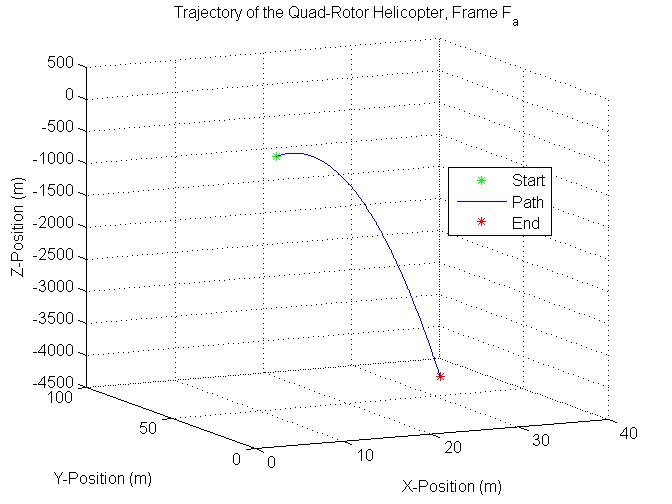
\includegraphics[width=.30\textwidth]{trajnoforcealpha50}
    \caption{Trajectory of the quad-rotor helicopter for Simulation $\#1$}
    \label{fig:trajnoforcealpha50}
\end{figure}

\begin{figure}[ht!!!!]
    \centering
        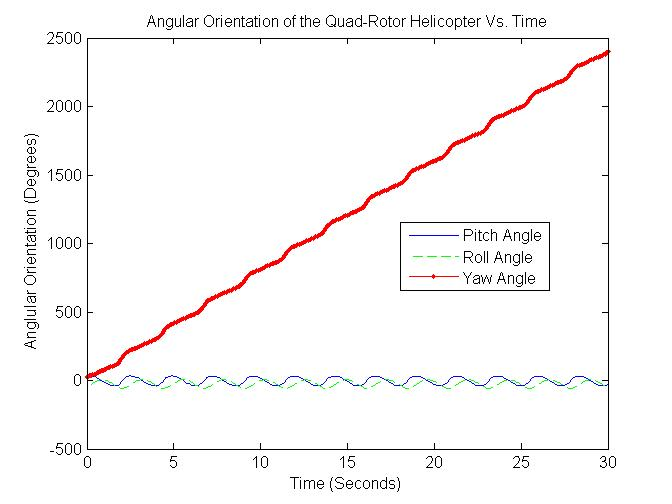
\includegraphics[width=.30\textwidth]{angoriennoforcealpha50}
    \caption{Angular orientation of the quad-rotor helicopter for Simulation $\#1$, $\dot{\alpha}$ = $50$ rev/s}
    \label{fig:angoriennoforcealpha50}
\end{figure}

\begin{figure}[ht!!!!]
    \centering
        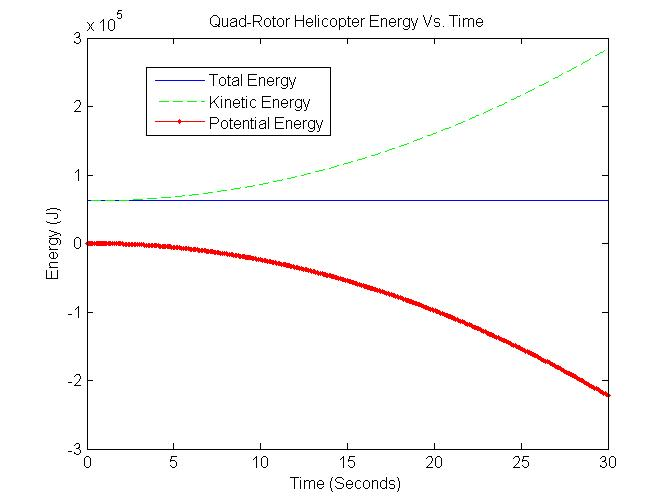
\includegraphics[width=.30\textwidth]{energynoforcealpha50}
    \caption{Energy of the quad-rotor helicopter for Simulation $\#1$}
    \label{fig:energynoforcealpha50}
\end{figure}

As one can see, the quad-rotor helicopter does experience free-fall behavior and its Euler-angle positions exhibit oscillatory behavior. Clearly, the total energy $E_{\mathcal{S}_w/a}$ remains constant with time as expected. This supports the notion that the kinematics and dynamics were derived and computed correctly. Also, as the helicopter falls, its potential energy $U_{\mathcal{S}_w}$ is transfered to its kinetic energy $T_{\mathcal{S}_w/a}$ in accordance with conservative-force-only (gravity) physics. 

Next, The relevant plots of all Simulation $\#2$ are displayed in Figures \ref{fig:angoriennoforcealpha500} through \ref{fig:angoriennoforcealpha5000}:

\begin{figure}[ht!!!!]
    \centering
        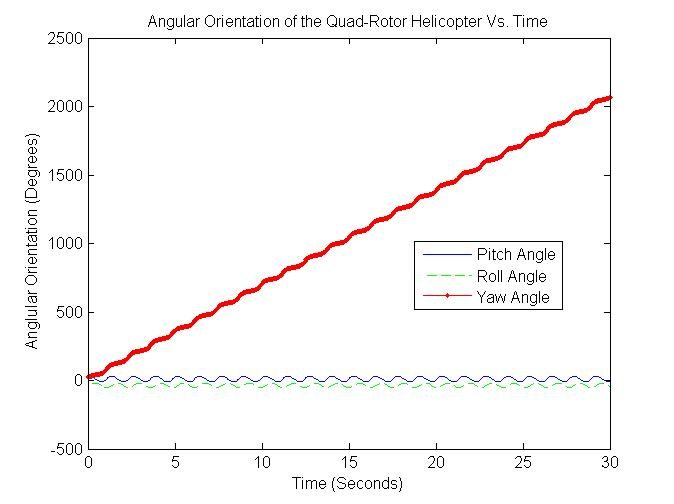
\includegraphics[width=.30\textwidth]{angoriennoforcealpha500}
    \caption{Angular orientation of the quad-rotor helicopter for Simulation $\#2$, $\dot{\alpha}$ = $500$ rev/s}
    \label{fig:angoriennoforcealpha500}
\end{figure}

\begin{figure}[ht!!!!]
    \centering
        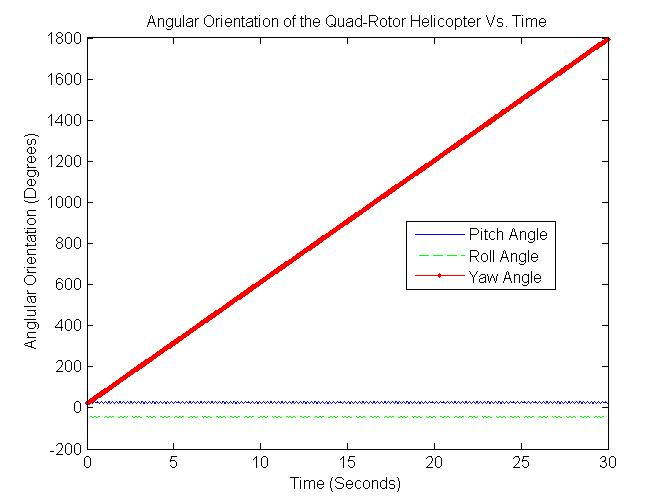
\includegraphics[width=.30\textwidth]{angoriennoforcealpha5000}
    \caption{Angular orientation of the quad-rotor helicopter for Simulation $\#2$, $\dot{\alpha}$ = $5000$ rev/s}
    \label{fig:angoriennoforcealpha5000}
\end{figure}

The oscillatory behavior of the Euler-angle positions is attenuated as the value of $\dot{\alpha}$ increases. This is not surprising because as $\dot{\alpha}$ increases, $\underline{h}^{\mathcal{R}c/a}_{b}$ increases, which, for a given net moment $\underrightarrow{m}^{\mathcal{S}c}$, the angular velocity component rates $\underline{\dot{\omega}}^{ba}_b$ decrease as per Equations \ref{eq:E2L1} and \ref{eq:E2L2}. Hence, the Euler-angle $rates$ are less susceptible to change as $\dot{\alpha}$ increases which explains their attenuated behavior for large $\dot{\alpha}$ values. 

\pagebreak
Last, The relevant plots of all Simulation $\#3$ are displayed in Figures \ref{fig:trajcontrollaw} through \ref{fig:energycontrollaw}:

\begin{figure}[ht!!!!]
    \centering
        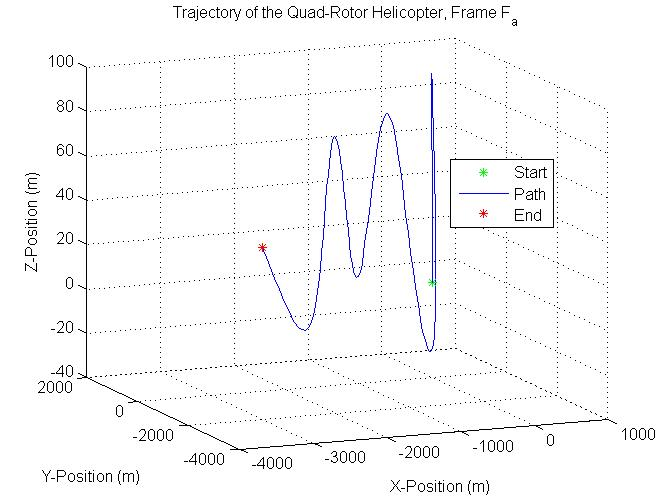
\includegraphics[width=.30\textwidth]{trajcontrollaw}
    \caption{Trajectory of the quad-rotor helicopter for Simulation $\#3$}
    \label{fig:trajcontrollaw}
\end{figure}

\begin{figure}[ht!!!!]
    \centering
        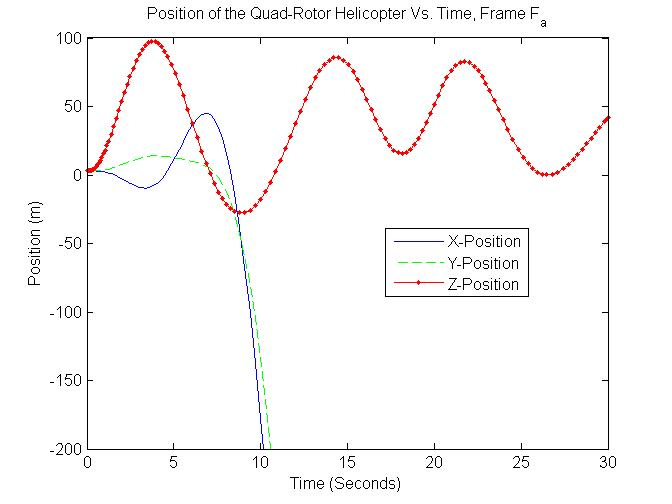
\includegraphics[width=.30\textwidth]{poscontrollaw}
    \caption{Position coordinates of the quad-rotor helicopter for Simulation $\#3$}
    \label{fig:poscontrollaw}
\end{figure}

\begin{figure}[ht!!!!]
    \centering
        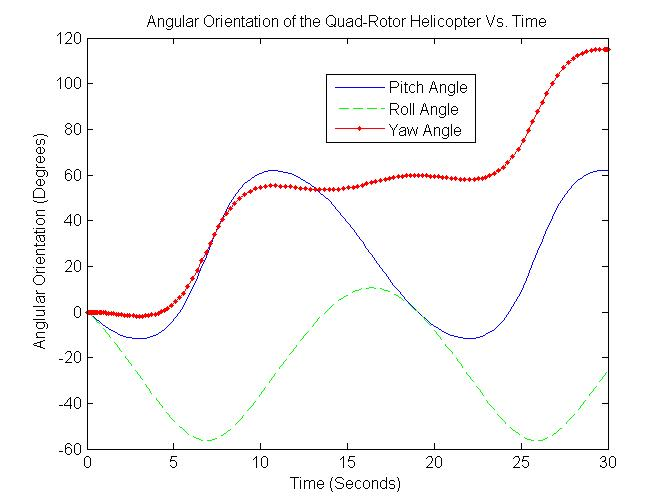
\includegraphics[width=.30\textwidth]{angoriencontrollaw}
    \caption{Angular orientation of the quad-rotor helicopter for Simulation $\#3$}
    \label{fig:angoriencontrollaw}
\end{figure}

\begin{figure}[ht!!!!]
    \centering
        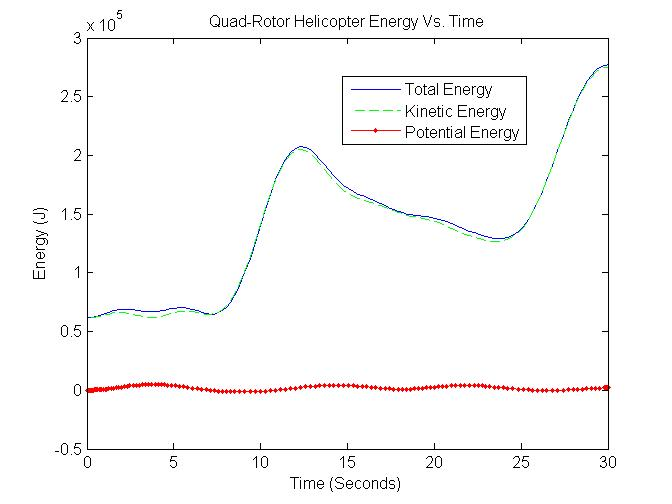
\includegraphics[width=.30\textwidth]{energycontrollaw}
    \caption{Energy of the quad-rotor helicopter for Simulation $\#3$}
    \label{fig:energycontrollaw}
\end{figure}

\pagebreak
Looking at Figure \ref{fig:poscontrollaw}, one can observe that the proportional control law is affecting the behavior of the quad-rotor helicopter in that its height $z_c$ oscillates about the desired height of $z_{des}=50$ meters. However, the helicopter never converges to the desired height due to a fundamental flaw of the control law. Whenever the helicopter reaches the desired height, the control law orders the four rotors to not produce any lift force above their base lift forces. Hence, there is nothing driving the helicopter to remain at the desired height once it gets there. Any non-zero velocity or non-level orientation signifies that the helicopter will move away from the desired height. It should be noted that without the control law, the helicopter simply falls downward. 

\section{Conclusion}
In this document, the kinematics and dynamics of a quad-rotor helicopter were modeled using a Newton-Euler approach. Equations of motion for the helicopter's $13$ states were derived which were then integrated using Matlab's $ode45()$ command. Three simulations were conducted which gave insight into the dynamics of the quad-rotor helicopter and how it behaved. Overall, much was learned in this project and it was very enjoyable. 
\bibliographystyle{IEEEtran}
\bibliography{540_refs}

\end{document}


